\section{Case Study: Lorenz System}

The Lorenz system is defined by
\begin{align*}
	\dot x &= \sigma (y-x)\\
	\dot y &= x(\rho-z)-y\\
	\dot z &= xy-\beta z \text,
\end{align*}
where $\sigma = \beta = 0.1$ and $\rho$ is the variable parameter.

As a reduction operator for the creation of the bifurcation diagram
\[
	\mathbf y \mapsto \{||\mathbf y(t) - \mathbf a||\ |\ t \in [0,2\pi),\ \mathbf y_3(t) = \rho + 7\}
\]
is used, where $\mathbf a = (\sqrt{\beta(\rho-1)}, \sqrt{\beta(\rho-1)}, \rho-1)^T$ is one of the fixed points of the system.
It maps a solution to the distances of its intersections with the $z = \rho+7$ plane to the fixed point $\mathbf a$.
This particular choice was made empirically, as most other choices result in changing numbers of intersections for single solution branches, too many intersections or result in many lines overlapping one another.

The system features stable periodic solutions for $\rho \in \{99.65, 100.5, 160, 350\}$.
These values are used as starting points for the creation of the bifurcation diagram.
The general process of finding a stable solution, tracing it to a bifurcation point or until otherwise satisfied, doubling the period and finding period doubling bifurcations is the same as for the Rössler system.

See figures \ref{fig:lorenzfull}, \ref{fig:lorenzcut} for visual results.
The tracing of the solutions for $\rho \to 0$ had to be suspended, because it became too slow to be practical.
See the discussion in \autoref{sec:outro} for details.

\newgeometry{top=0cm}

\begin{figure}
\centering\makebox[0pt]{\rotatebox{90}{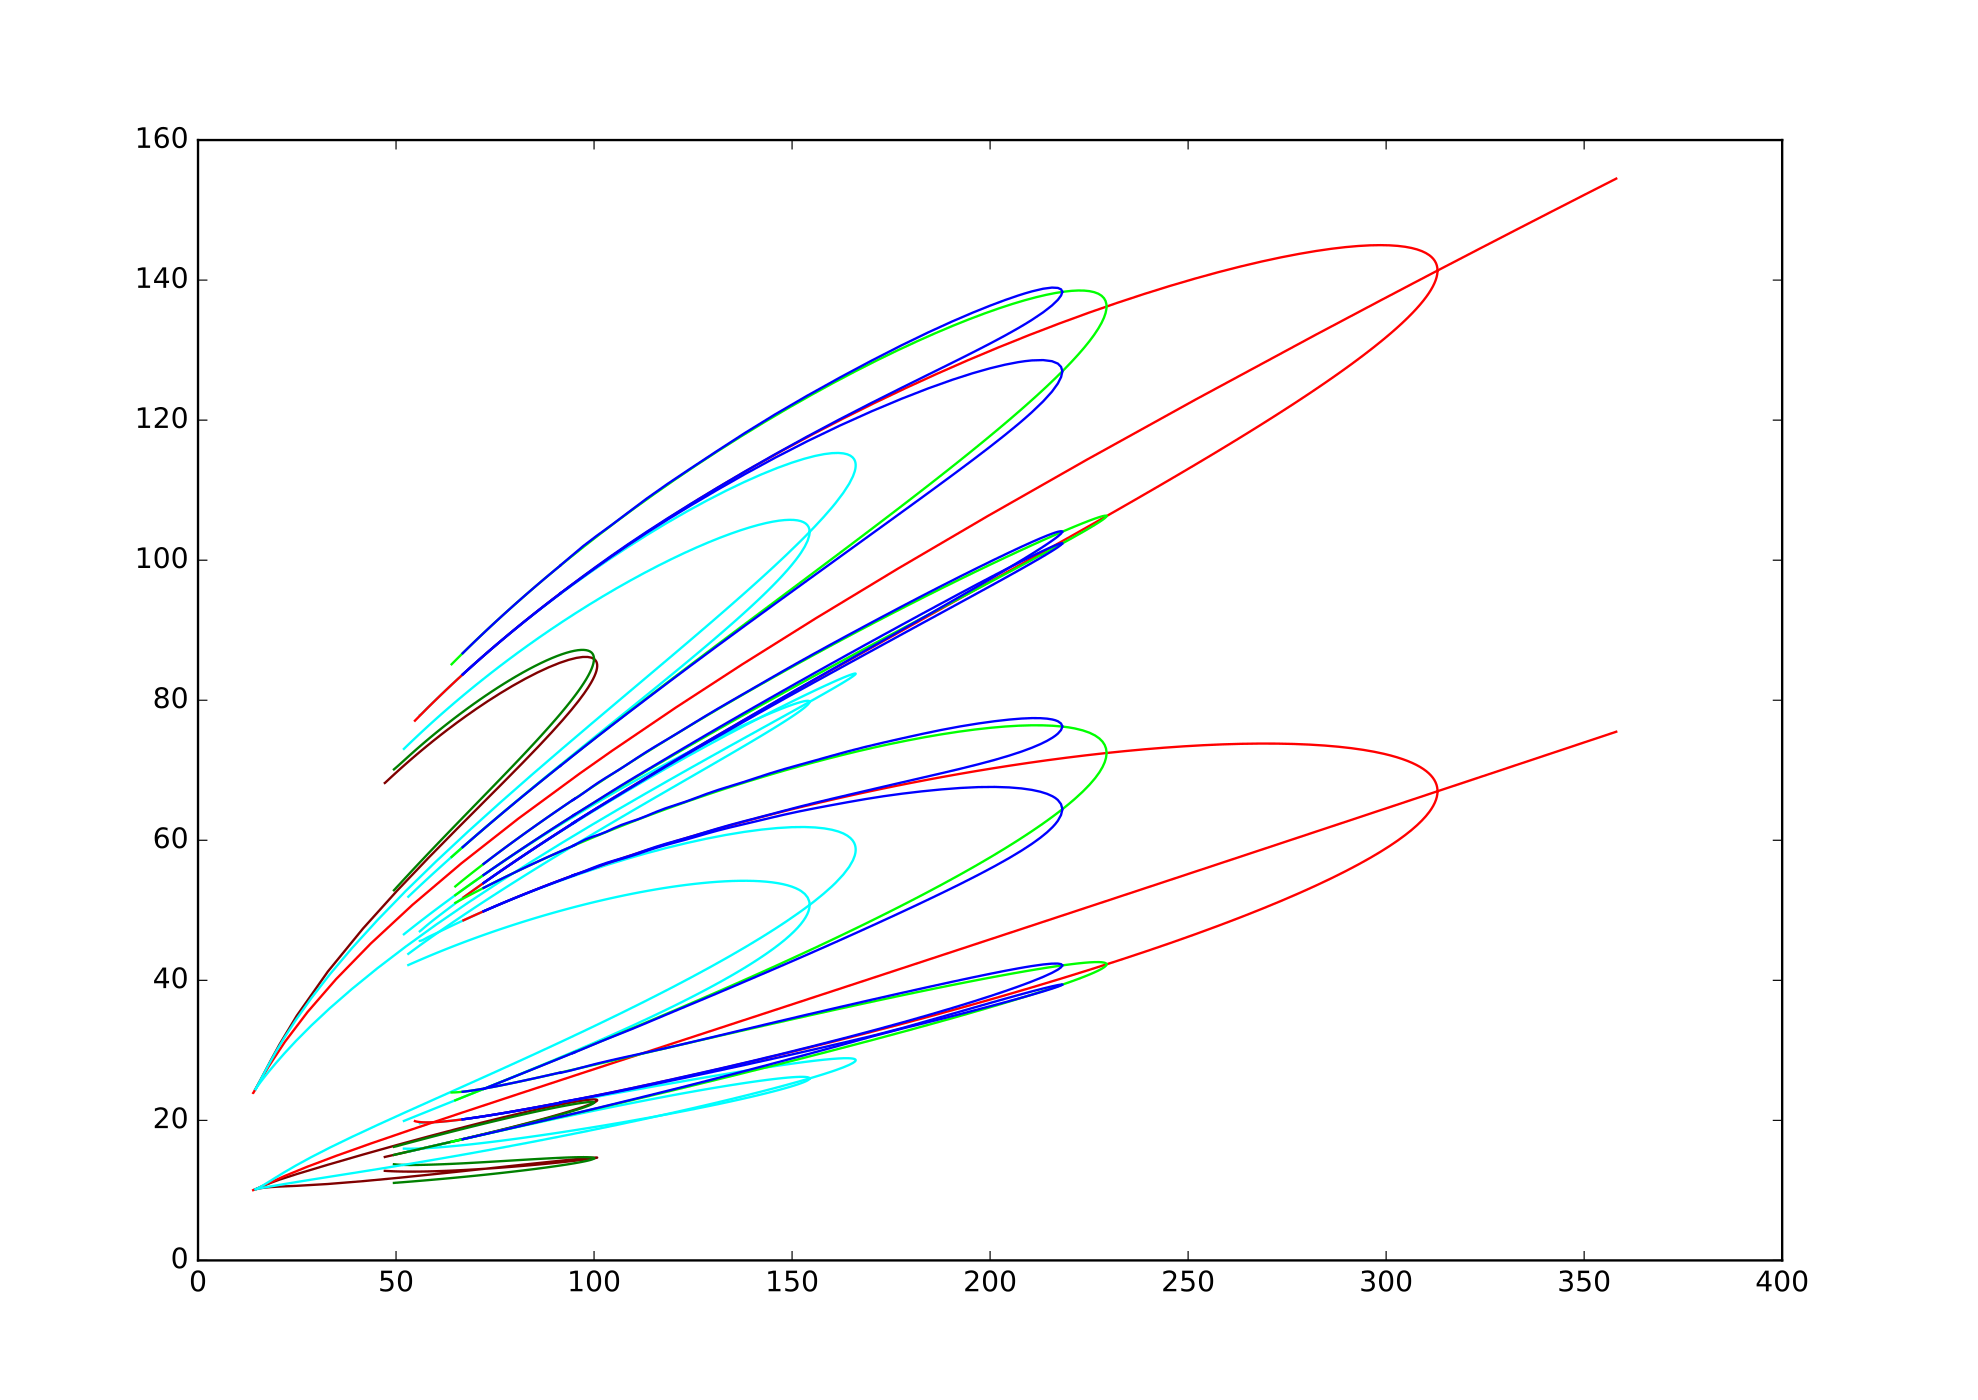
\includegraphics{img/lorenzoverview.png}}}
\caption{
	An overview of the Lorenz bifurcation diagram.
}
\label{fig:lorenzfull}
\end{figure}


\begin{figure}
\centering\makebox[0pt]{\rotatebox{90}{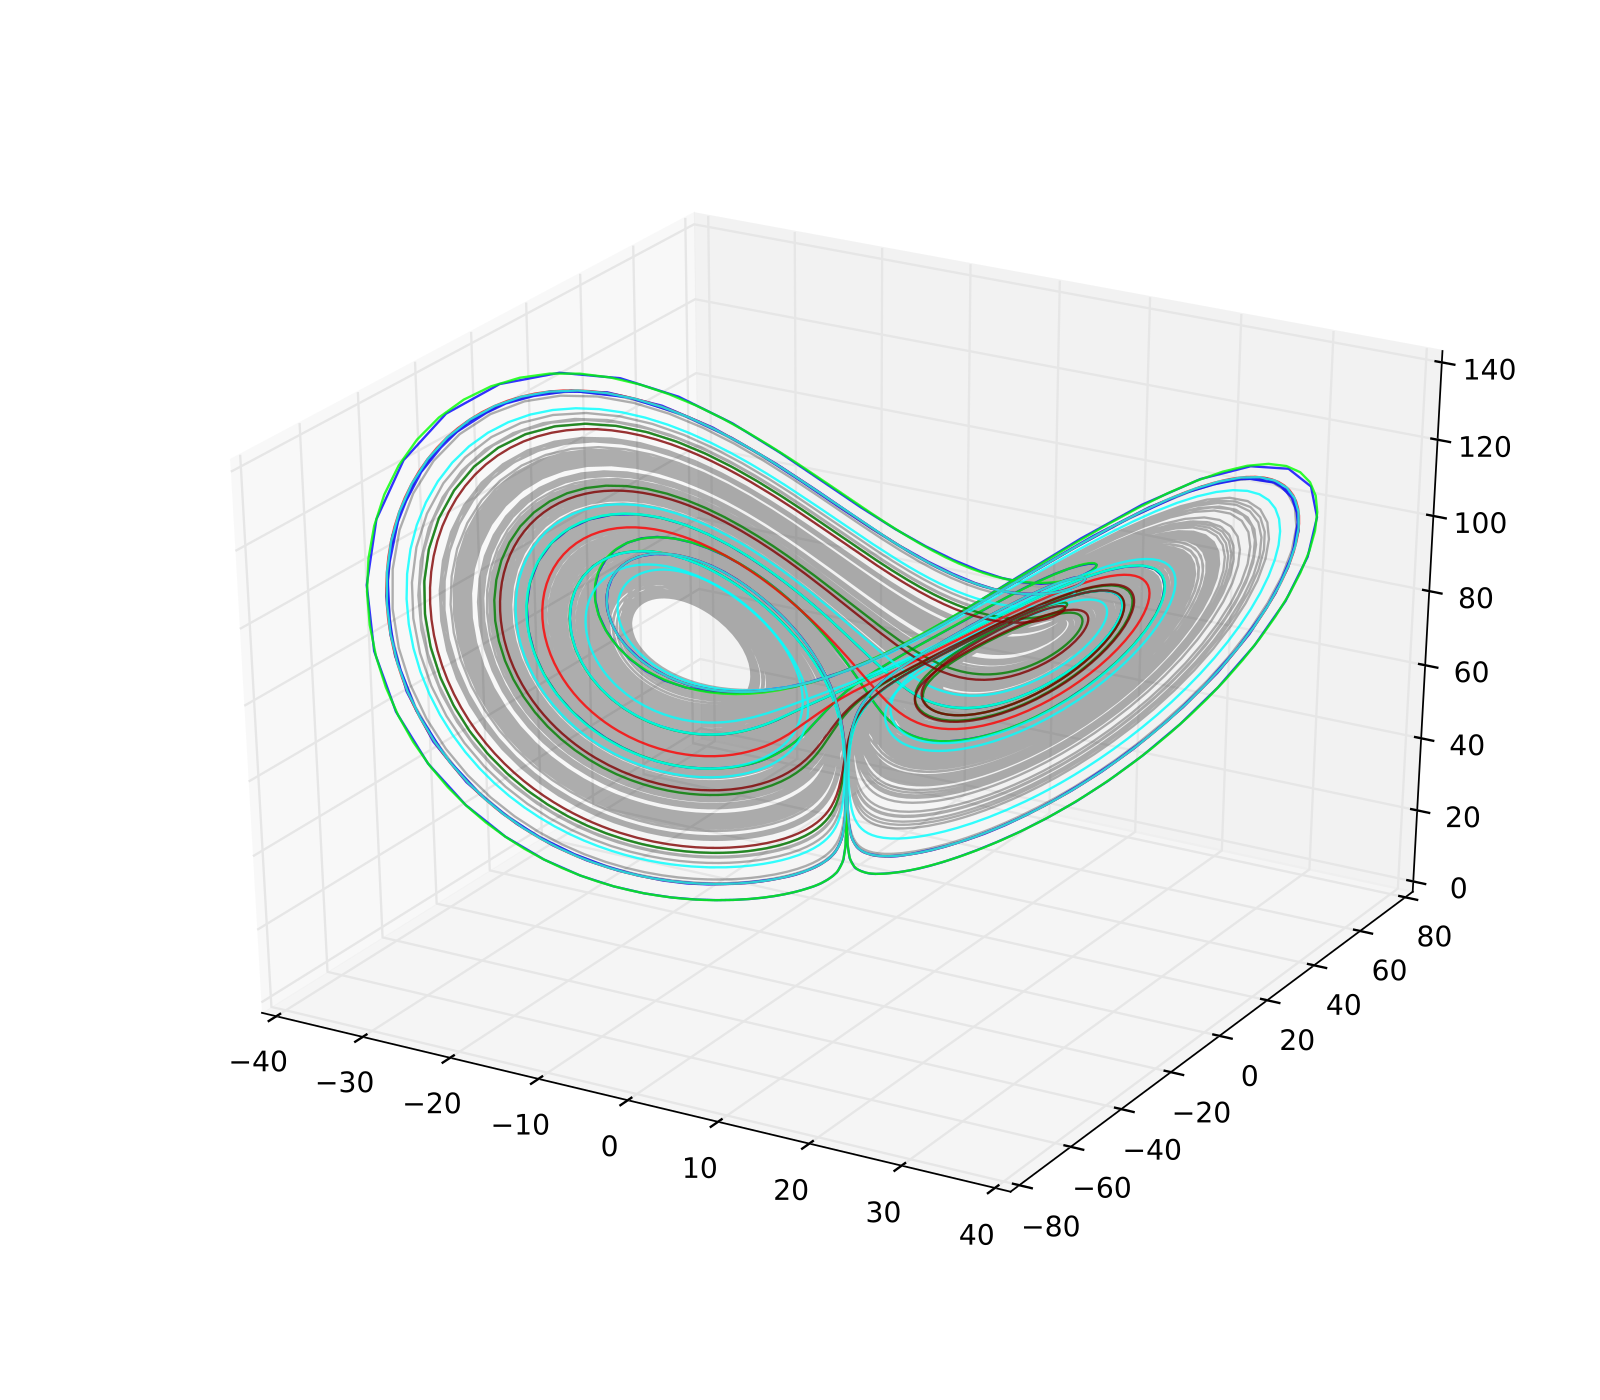
\includegraphics{img/lorenzcut80.png}}}
\caption{
	The periodic orbits for $\rho=80$, together with an underlying trajectory obained through forward intergration (grey) in phase-space. 
	The colors of the periodic solutions match the bifurcation diagram.
}
\label{fig:lorenzcut}
\end{figure}

\restoregeometry